\documentclass{article}

\usepackage{listings}
\usepackage{color}
\usepackage{graphicx}
\usepackage{float}

\title{Lab 2: Simple Parallel IO}
\date{October 10, 2017}
\author{Matthew Friedman 861151348\\Souradeep Bhattacharya 861105938\\EE128 Section: 021}

\definecolor{dkgreen}{rgb}{0,0.6,0}
\definecolor{gray}{rgb}{0.5,0.5,0.5}
\definecolor{mauve}{rgb}{0.58,0,0.82}

\lstset{frame=tb,
	language=C,
	aboveskip=3mm,
	belowskip=3mm,
	showstringspaces=false,
	columns=flexible,
	basicstyle={\small\ttfamily},
	numbers=none,
	numberstyle=\tiny\color{gray},
	keywordstyle=\color{blue},
	commentstyle=\color{dkgreen},
	stringstyle=\color{mauve},
	breaklines=true,
	breakatwhitespace=true,
	tabsize=4
}

\begin{document}
\maketitle

\section*{Abstract}
The objective of this lab was to become familiar with the development environment for 9S12DG256-based system. The second objective was to learn hardware/software techniques for developing, testing, and debugging microcontroller-based digital systems. The second part of the experiment was to create an 8-bit, bi-directional, binary counter and a hot-rotator. 
\section*{Experiment System Specification}
\paragraph{Part 1}
This section is a step-by-step tutorial to learn how to (i) connect to the Dragon12-JR evaluation board to the development PC, (ii) use RealTerm to interact with the evaluation board, and (iii) develop a program in Freescale CodeWarrior. This code blinks the 7-segment LED of the evaluation board.
\paragraph{Part 2}
This section of the experiment requires us to build (i) an 8-bit, bi-directional, binary counter, and (ii) an 8-bit, bi-directional, one-hot rotator. Both of them should run at 1Hz by software delay. The counting direction (0:upwards or 1:downwards) for the counter, and the rotating direction (0:left or 1:right) for the rotator. The previous signals are given by 2-bit DIP switch. The states of the counter and the hot rotator should be displayed by the two 8-bit LED bars.

\section*{Block Diagram and Hardware Design}
\subsection*{Part 2}
\begin{figure}[H]
	\centering
	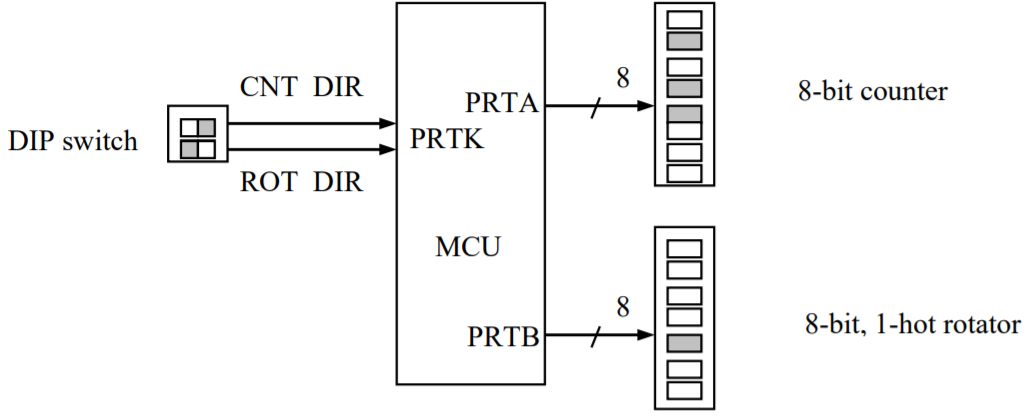
\includegraphics[width=1\textwidth]{Part2_Block_Diagram}
\end{figure}
\section*{Detailed Schematic Diagram}
\subsection*{Part 2}
\begin{figure}[H]
	\centering
	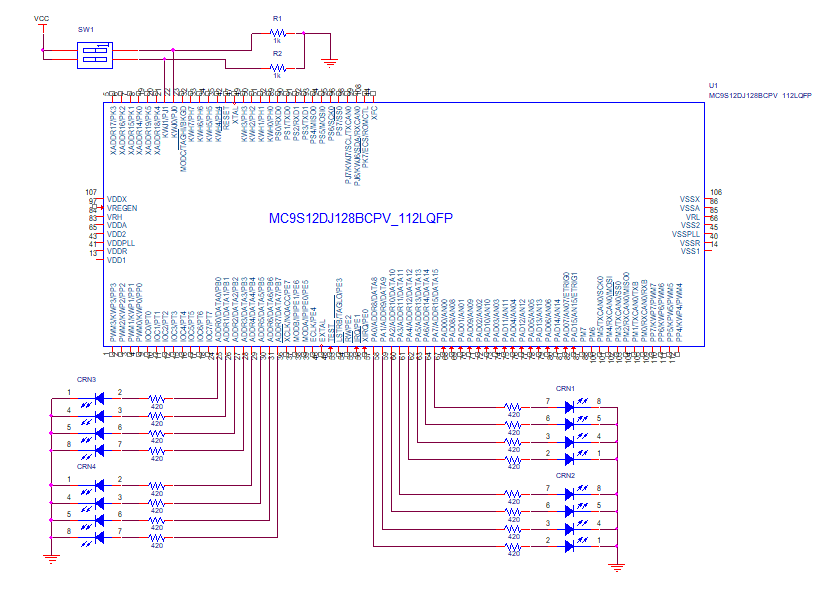
\includegraphics[width=1\textwidth]{Lab2_part2}
\end{figure}
\section*{High Level Description of the Software}
\subsection*{Part 2}
The program increments or decrements a counter one time per second depending on on the state of a DIP switch connected to K0. The state of the counter is displayed on a LED bar connected to Port A. We also have a one-hot rotator connected to Port B which rotates left or right depending on the state of another DIP switch connected to K1.
\section*{Program Listings}
\subsection*{Part 2 C Code}
\begin{lstlisting}
#include <hidef.h>      /* common defines and macros */
#include <mc9s12dg256.h>     

//declare variables
int cnt_dir = 0;
int rot_dir = 0;
int cnt_val = 0;
int rot_val = 1;
long i = 0;
int rot_count = 0;

void main(void) 
{
	//setup ports
	DDRA = 255;   //counter port
	DDRB = 255;   //rotator port
	DDRK = 0;     //dip switch port

	//loop forever
	while(1) 
	{
		//SW delay, i must be type "long"
		for (i=0;i<100000;i++);   //100000 is 10 times per sec, 1000000 is 1 sec

		//read directions from port k
		cnt_dir = PORTK & 1;
		rot_dir = PORTK & 2;

		//set values depending on port k input
		if(cnt_dir) 
		{
			cnt_val++;
		} 
		else
		{
			cnt_val--;
		}
		if(rot_dir) 
		{
			if(rot_count < 7) 
			{
				rot_count++;
				rot_val = rot_val << 1;
			} 
			else
			{
				rot_count = 0;
				rot_val = 1;
			}
		} 
		else
		{
			if(rot_count > 0) 
			{
				rot_count--;
				rot_val = rot_val >> 1;
			} 
			else
			{
				rot_count = 7;
				rot_val = 128;
			}
		}

		//set port values
		PORTA = cnt_val;
		PORTB = rot_val;   
	}
}
\end{lstlisting}
\subsection*{Part 2 Project PRM}
\begin{lstlisting}
NAMES END
SECTIONS
	MY_RAM = READ_WRITE 0x1000 TO 0x1FFF; /* 4095 bytes of data */
	MY_PSEUDO_ROM = READ_ONLY 0x2000 TO 0x3FFF; /* 8191 bytes of code */
END

PLACEMENT
	_PRESTART,
	STARTUP,
	ROM_VAR,
	STRINGS,
	DEFAULT_ROM, NON_BANKED,
	COPY INTO MY_PSEUDO_ROM;
	DEFAULT_RAM INTO MY_RAM;
END

STACKSIZE 0x100
\end{lstlisting}
\section*{Technical Problems}
\paragraph{No Lights}
We had the code set up and we could not see any blinking lights. In order to solve this we just had to remake the code. We also had to change the direction of the LED bar. The corner of the LED bar indicates positive end.

\paragraph{Garbled Communications}
We had lost communication to the board via RealTerm. We just had to switch to a different baud rate and then switch back to 9600 and it started working again. We also found out that every time we reset the board we need to reselect the file.

\section*{Answers To Questions}
\begin{enumerate}
	\item The size on Windows is 542 bytes. The size on the microcontroller is 139 bytes. This can be a result of how Windows stores the files on the disk.
	
	\item The two do not change their states at the exact same time. Because of how the code executes one of the states must change before the other. In our code the counter changes states right before the rotator. Because of the speed at which the microcontroller runs it gives the illusion of occurring at the same time. This is evidenced below in the captured result of the oscilloscope. 
	\begin{figure}[H]
		\centering
		\includegraphics[width=1\textwidth]{Q2}
	\end{figure}

	\item With out the software delay the program ran at 181.8KHz. Shown below:
	\begin{figure}[H]
		\centering
		\includegraphics[width=1\textwidth]{Q3}
	\end{figure}
\end{enumerate}

\section*{Conclusion}
Barring some small technical challenges we were able to create the system specified by the lab requirements. This whole lab really made me and my partner appreciate Arduino ability to make the microcontroller market accessible to the general public.
\end{document}